\documentclass[border=5pt]{standalone}
\usepackage{tikz}
\usetikzlibrary{arrows.meta, positioning, calc, decorations.pathreplacing}
\usepackage{xcolor}

% Brand colors
\definecolor{Garnet}{HTML}{73000A}
\definecolor{NinetyBlack}{HTML}{363636}
\definecolor{SeventyBlack}{HTML}{5C5C5C}
\definecolor{FiftyBlack}{HTML}{A2A2A2}
\definecolor{ThirtyBlack}{HTML}{C7C7C7}
\definecolor{TenBlack}{HTML}{ECECEC}
\definecolor{Atlantic}{HTML}{466A9F}
\definecolor{Congaree}{HTML}{1F414D}
\definecolor{Horseshoe}{HTML}{65780B}
\definecolor{Sandstorm}{HTML}{FFF2E3}

\tikzset{every node/.append style={rounded corners=0pt}}

\begin{document}
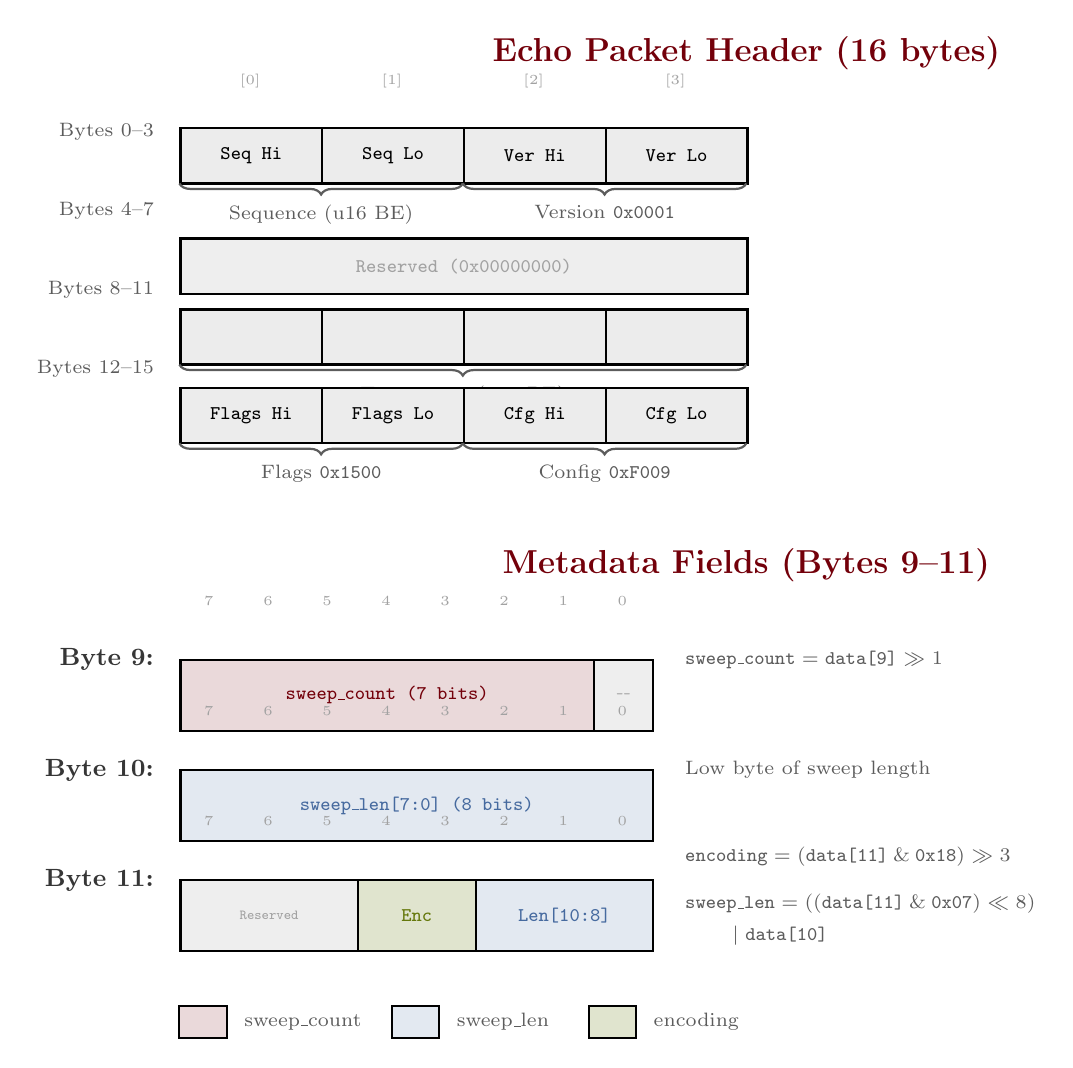
\begin{tikzpicture}[
    byte/.style={draw, thick, minimum width=0.9cm, minimum height=0.7cm, anchor=west, font=\ttfamily\scriptsize},
    bitcell/.style={draw, thick, minimum width=0.75cm, minimum height=0.9cm, anchor=west, font=\ttfamily\scriptsize, align=center},
    lbl/.style={font=\small\bfseries, color=NinetyBlack},
    annot/.style={font=\scriptsize, color=SeventyBlack},
]

% ── 16-Byte Header (top section) ──
\node[font=\bfseries\large, color=Garnet] at (7.2, 8.5) {Echo Packet Header (16 bytes)};

% Row labels
\node[annot, anchor=east] at (-0.2, 7.5) {Bytes 0--3};
\node[annot, anchor=east] at (-0.2, 6.5) {Bytes 4--7};
\node[annot, anchor=east] at (-0.2, 5.5) {Bytes 8--11};
\node[annot, anchor=east] at (-0.2, 4.5) {Bytes 12--15};

% Row 1: Bytes 0-3
\node[byte, fill=TenBlack, minimum width=1.8cm] (b0) at (0, 7.2) {Seq Hi};
\node[byte, fill=TenBlack, minimum width=1.8cm] (b1) at (1.8, 7.2) {Seq Lo};
\node[byte, fill=TenBlack, minimum width=1.8cm] (b2) at (3.6, 7.2) {Ver Hi};
\node[byte, fill=TenBlack, minimum width=1.8cm] (b3) at (5.4, 7.2) {Ver Lo};
\draw[decorate, decoration={brace, amplitude=4pt, mirror}, thick, SeventyBlack]
    (0, 6.85) -- (3.6, 6.85) node[midway, below=4pt, font=\scriptsize, color=SeventyBlack] {Sequence (u16 BE)};
\draw[decorate, decoration={brace, amplitude=4pt, mirror}, thick, SeventyBlack]
    (3.6, 6.85) -- (7.2, 6.85) node[midway, below=4pt, font=\scriptsize, color=SeventyBlack] {Version \texttt{0x0001}};

% Row 2: Bytes 4-7
\node[byte, fill=ThirtyBlack!30, minimum width=7.2cm] (b4) at (0, 5.8) {\color{FiftyBlack}Reserved (\texttt{0x00000000})};

% Row 3: Bytes 8-11
\node[byte, fill=TenBlack, minimum width=1.8cm] (b8) at (0, 4.9) {};
\node[byte, fill=TenBlack, minimum width=1.8cm] (b9) at (1.8, 4.9) {};
\node[byte, fill=TenBlack, minimum width=1.8cm] (b10) at (3.6, 4.9) {};
\node[byte, fill=TenBlack, minimum width=1.8cm] (b11) at (5.4, 4.9) {};
\draw[decorate, decoration={brace, amplitude=4pt, mirror}, thick, SeventyBlack]
    (0, 4.55) -- (7.2, 4.55) node[midway, below=4pt, font=\scriptsize, color=SeventyBlack] {Timestamp (u32 BE)};

% Row 4: Bytes 12-15
\node[byte, fill=TenBlack, minimum width=1.8cm] (b12) at (0, 3.9) {Flags Hi};
\node[byte, fill=TenBlack, minimum width=1.8cm] (b13) at (1.8, 3.9) {Flags Lo};
\node[byte, fill=TenBlack, minimum width=1.8cm] (b14) at (3.6, 3.9) {Cfg Hi};
\node[byte, fill=TenBlack, minimum width=1.8cm] (b15) at (5.4, 3.9) {Cfg Lo};
\draw[decorate, decoration={brace, amplitude=4pt, mirror}, thick, SeventyBlack]
    (0, 3.55) -- (3.6, 3.55) node[midway, below=4pt, font=\scriptsize, color=SeventyBlack] {Flags \texttt{0x1500}};
\draw[decorate, decoration={brace, amplitude=4pt, mirror}, thick, SeventyBlack]
    (3.6, 3.55) -- (7.2, 3.55) node[midway, below=4pt, font=\scriptsize, color=SeventyBlack] {Config \texttt{0xF009}};

% Byte offset labels above
\foreach \i/\off in {0/0, 1/1, 2/2, 3/3} {
    \node[font=\tiny, color=FiftyBlack, above=1pt] at (0.9 + \i*1.8, 7.9) {[\off]};
}

% ── Metadata Zoom: Bytes 9-11 ──
\node[font=\bfseries\large, color=Garnet] at (7.2, 2.0) {Metadata Fields (Bytes 9--11)};

% Byte 9 bit breakdown
\node[lbl, anchor=east] at (-0.2, 0.8) {Byte 9:};
\foreach \i/\v in {0/7, 1/6, 2/5, 3/4, 4/3, 5/2, 6/1, 7/0} {
    \node[font=\tiny, color=FiftyBlack] at (0.375 + \i*0.75, 1.55) {\v};
}
\node[bitcell, fill=Garnet!15, minimum width=5.25cm] (s9hi) at (0, 0.35) {\color{Garnet}\textbf{sweep\_count} (7 bits)};
\node[bitcell, fill=ThirtyBlack!30, minimum width=0.75cm] (s9lo) at (5.25, 0.35) {\color{FiftyBlack}\tiny --};
\node[annot, anchor=west] at (6.3, 0.8) {$\texttt{sweep\_count} = \texttt{data[9]} \gg 1$};

% Byte 10 bit breakdown
\node[lbl, anchor=east] at (-0.2, -0.6) {Byte 10:};
\foreach \i/\v in {0/7, 1/6, 2/5, 3/4, 4/3, 5/2, 6/1, 7/0} {
    \node[font=\tiny, color=FiftyBlack] at (0.375 + \i*0.75, 0.15) {\v};
}
\node[bitcell, fill=Atlantic!15, minimum width=6.0cm] (s10) at (0, -1.05) {\color{Atlantic}\textbf{sweep\_len[7:0]} (8 bits)};
\node[annot, anchor=west] at (6.3, -0.6) {Low byte of sweep length};

% Byte 11 bit breakdown
\node[lbl, anchor=east] at (-0.2, -2.0) {Byte 11:};
\foreach \i/\v in {0/7, 1/6, 2/5, 3/4, 4/3, 5/2, 6/1, 7/0} {
    \node[font=\tiny, color=FiftyBlack] at (0.375 + \i*0.75, -1.25) {\v};
}
\node[bitcell, fill=ThirtyBlack!30, minimum width=2.25cm] (s11rsv) at (0, -2.45) {\color{FiftyBlack}\tiny Reserved};
\node[bitcell, fill=Horseshoe!20, minimum width=1.5cm] (s11enc) at (2.25, -2.45) {\color{Horseshoe}\textbf{Enc}};
\node[bitcell, fill=Atlantic!15, minimum width=2.25cm] (s11len) at (3.75, -2.45) {\color{Atlantic}\textbf{Len[10:8]}};
\node[annot, anchor=west] at (6.3, -1.7) {$\texttt{encoding} = (\texttt{data[11]} \mathbin{\&} \texttt{0x18}) \gg 3$};
\node[annot, anchor=west] at (6.3, -2.3) {$\texttt{sweep\_len} = ((\texttt{data[11]} \mathbin{\&} \texttt{0x07}) \ll 8)$};
\node[annot, anchor=west] at (6.9, -2.7) {$\mathbin{|}\; \texttt{data[10]}$};

% Legend
\node[draw, thick, fill=Garnet!15, minimum width=0.6cm, minimum height=0.4cm] at (0.3, -3.8) {};
\node[annot, anchor=west] at (0.7, -3.8) {sweep\_count};
\node[draw, thick, fill=Atlantic!15, minimum width=0.6cm, minimum height=0.4cm] at (3.0, -3.8) {};
\node[annot, anchor=west] at (3.4, -3.8) {sweep\_len};
\node[draw, thick, fill=Horseshoe!20, minimum width=0.6cm, minimum height=0.4cm] at (5.5, -3.8) {};
\node[annot, anchor=west] at (5.9, -3.8) {encoding};

\end{tikzpicture}
\end{document}
